\chapter{Methods and Materials}\label{ch:3}

\section{Architecture}

MOCHI separates the control plane from the data plane (Figure 1). The control plane decides what to do next; the data plane performs every computation that appears in the report. The manager is the only agent that sees the user's instruction; it retrieves a reasoning template by TF-IDF similarity, decomposes the task into four stages and delegates execution. The developer executes a stage program and may only change parameters from a whitelist. The critic runs a scenario-specific, deterministic audit and then asks the language model for a verdict; the stricter of the two wins, so the model cannot waive a failed control. When the audit reports a missing capability, the tool-creation agent researches, writes, tests and registers a new tool, and the affected stage is re-run.

\begin{figure}[htbp]
\centering
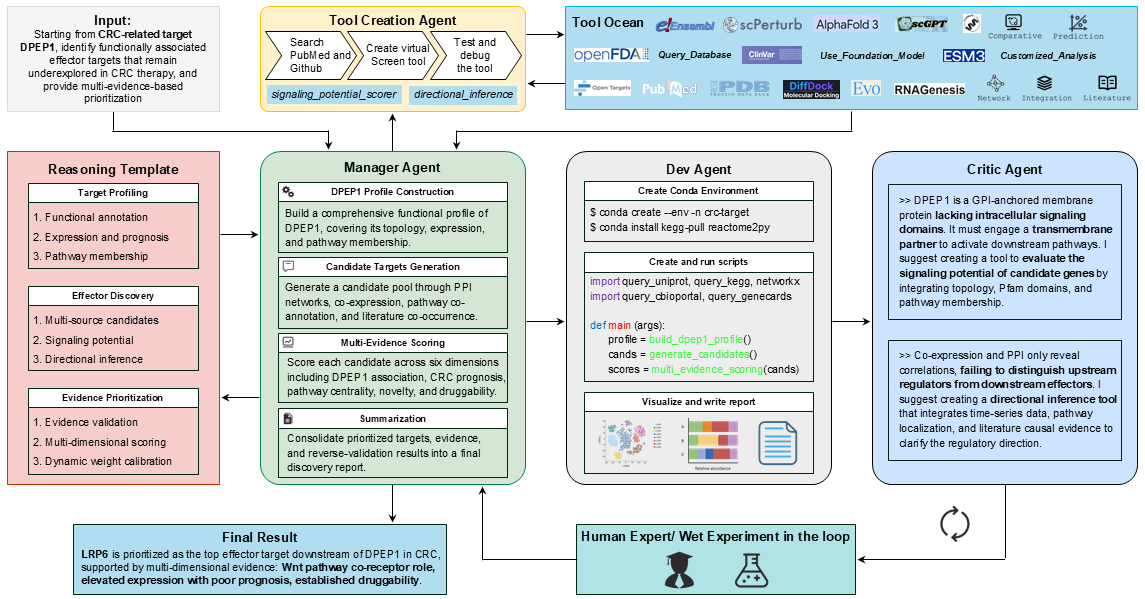
\includegraphics[width=0.99\textwidth]{figures/fig_workflow_ref.png}
\caption{The target-discovery workflow. The manager decomposes the DPEP1 task into profile construction, candidate generation, multi-evidence scoring and summarisation; the developer runs the stage programs and writes the artefacts; the critic audits each stage and asks for a new tool when a capability is missing; the tool-creation agent searches, builds and tests that tool before the stage is re-run. The final panel shows the hypothesis that the wet lab then tested; the quantitative evidence behind each step is reported in Section 4.}
\end{figure}

\section{Agents and their contracts}

Every agent call is a JSON contract, and the orchestrator parses only JSON. This is what allows the same agent classes to run against a real model, a local mock, or a rule-based engine: the contract, not the prose, carries the information.

\begin{table}[htbp]
\centering
\small
\caption{Agent contracts. The audit (Python) is evaluated separately from the verdict (model) and can override it.}
\begin{tabularx}{\textwidth}{l>{\raggedright\arraybackslash}X>{\raggedright\arraybackslash}X}
\hline
Call & Producer $\rightarrow$ consumer & Required fields \\
\hline
manager.plan & manager $\rightarrow$ orchestrator & stages\cite{r04} (name, goal, tools, criteria), hypotheses, reasoning \\
dev.plan & developer $\rightarrow$ stage program & steps, tools, parameter overrides (whitelisted) \\
critic.review & critic $\rightarrow$ manager & verdict (accept/revise/evolve), gaps, tool\_requests, weights \\
tool\_creation.design & tool creator $\rightarrow$ tool creator & tool name, algorithm, validation plan \\
manager.weights & manager $\rightarrow$ orchestrator & six weights summing to one \\
manager.synthesize & manager $\rightarrow$ report & narrative paragraph \\
\hline
\end{tabularx}

\end{table}

\section{Tool Ocean}

The Tool Ocean contains 46 deterministic tools in eleven categories (Table 4). Every tool returns a structured dictionary with an ok flag and a source string, never raises, and routes network access through one HTTP layer that caches responses for a week, retries with back-off, and appends the URL, parameters, status, latency and payload hash to provenance.jsonl. This single design decision is what makes the 'every number is traceable' claim in this report true.

\begin{table}[htbp]
\centering
\small
\caption{Tool Ocean by category. Counts exclude the runtime-created signalling-competence scorer.}
\begin{tabularx}{\textwidth}{l c >{\raggedright\arraybackslash}X}
\hline
Category & n & Representative tools \\
\hline
database & 12 & query\_uniprot, query\_opentargets\_associations, query\_cbioportal\_survival, query\_pubmed, query\_kegg\_pathways, resolve\_gene\_ids \\
chemistry & 6 & molecule\_properties, drugability\_score, query\_chembl\_target, query\_dgidb \\
literature & 5 & query\_pubmed\_cooccurrence, query\_pubmed\_novelty, citation\_network\_score \\
pathway / annotation & 8 & pathway\_coannotation, query\_quickgo, query\_interpro, pathway\_enrichment \\
network & 3 & query\_string, query\_intact, build\_ppi\_union \\
structure / sequence & 5 & fetch\_alphafold\_model, pocket\_geometry, conserve\_profile, primers, CDS mapping \\
retrosynthesis & 2 & one\_step\_disconnections, search\_route, route\_metrics \\
laboratory automation & 4 & parse\_protocol, compile\_sdl, validate\_sdl, simulate\_sdl \\
scoring & 1 & multi\_evidence\_scoring (plus the runtime-created competence scorer) \\
\hline
\end{tabularx}

\end{table}

\begin{figure}[htbp]
\centering
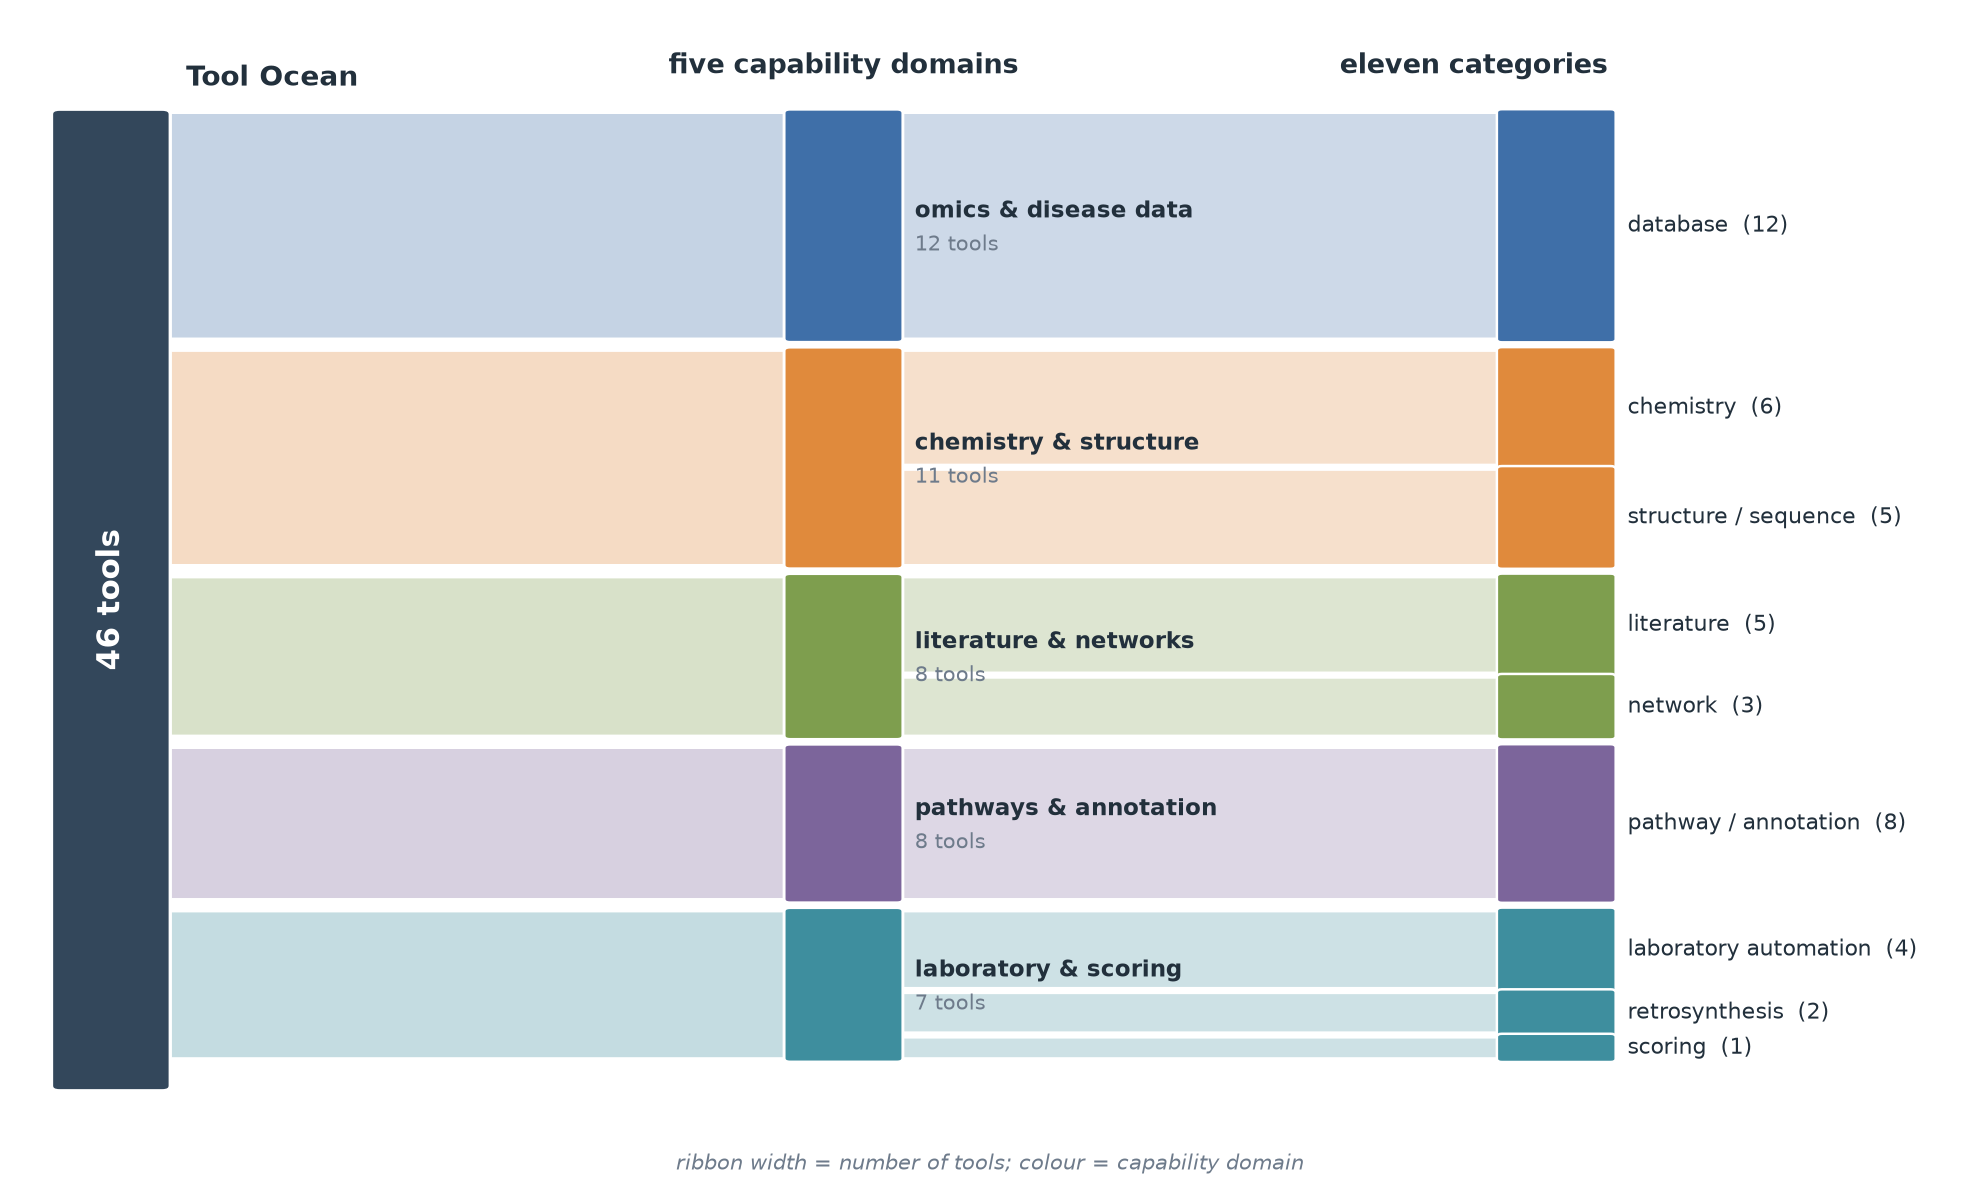
\includegraphics[width=0.99\textwidth]{figures/fig_sankey.png}
\caption{How the 46 tools of the Tool Ocean are distributed over five capability domains and the eleven categories. Ribbon width is proportional to the number of tools and the colour identifies the domain; the individual tools behind each category are listed in Table 4.}
\end{figure}

\section{Scenario adapters}

A scenario supplies four stage programs, an optional audit and an optional report renderer; nothing else changes. This is the entire mechanism by which MOCHI becomes a platform rather than a single-task agent. Table 5 summarises the stages.

\begin{table}[htbp]
\centering
\small
\caption{The four scenarios share the same four-stage skeleton.}
\begin{tabularx}{\textwidth}{l>{\raggedright\arraybackslash}X>{\raggedright\arraybackslash}X>{\raggedright\arraybackslash}X>{\raggedright\arraybackslash}X}
\hline
Stage & S1 target discovery & S2 enzyme design & S3 retrosynthesis & S4 protocol $\rightarrow$ SDL \\
\hline
Stage 1 & anchor profile: topology, expression, disease links & sequence, catalytic residues, AlphaFold model, homologs & target descriptors and functional-group inventory & sentence segmentation and typed step extraction \\
Stage 2 & candidate pool from PPI, co-expression, pathways, literature & all single substitutions within 12 A of the catalytic cluster & one-step disconnections from a curated template set & lowering to typed opcodes with SI units and devices \\
Stage 3 & signalling-competence scoring (created tool) & structure + chemistry + prior scoring & best-first AND-OR search to purchasable stock & static validation and bounded repair \\
Stage 4 & six-dimension ranking and evidence dossier & budgeted library, primers, hindcast & route ranking and literature benchmark & digital-twin simulation and corrupted-protocol benchmark \\
\hline
\end{tabularx}

\end{table}

\section{Decision models}

No stage delegates a computation to the language model. The models below are the actual decision rules; they were designed before the validation data were consulted and were not tuned on it.

Target discovery. Each candidate receives six dimension scores in [0,1] - association with the anchor, signalling competence, disease evidence, pathway centrality, novelty and druggability - and a weighted mean is taken over the dimensions that exist, multiplied by a coverage factor. Association combines physical interaction, expression co-variation, literature co-mention and specific pathway sharing with a noisy-OR, so that one strong channel is sufficient and absent channels do not dilute a real signal. Novelty is a saturating function of the number of PubMed records for the gene in the disease and overall, so a gene with no disease literature but 800 general papers is not counted as unexplored.

Enzyme design. A variant at position p with substitution wt$\rightarrow$mut receives score = leverage(d) $\times$ [0.55$\cdot$chemistry + 0.45$\cdot$prior] $\times$ (0.7 + 0.3$\cdot$packing) − 0.15$\cdot$conservation, where leverage = exp(−d/12) with d the minimum heavy-atom distance to the catalytic cluster, chemistry is a rescaled BLOSUM62 \cite{r15}, prior is the round-1 outcome for that position (hit 1.0 / reduced 0.5 / untested 0.5 / dead 0), packing penalises volume change and buried-glycine substitutions, and the conservation penalty comes from a Needleman-Wunsch alignment against 39 UniProt homologs.

Retrosynthesis. Six disconnection templates (amide, ester, aryl ether, N-alkylation, sulfonamide, nitro-to-amine interconversion) are applied by direct bond editing; the resulting fragments are sanitised, and a depth-limited best-first search terminates when every leaf is in a curated stock of commercially available building blocks \cite{r18,r20}.

Protocol compilation. A rule-based parser maps sentences to verbs and parameters, the compiler emits ten opcodes with SI units and device assignments, the validator checks vessel capacity, device temperature limits, unit completeness, ordering and flammable-solvent hazards, and the simulator produces a timeline on a digital twin of the platform.

\section{Audit, veto and self-evolution}

Each scenario defines a small set of hard checks (for example: was a sequence retrieved, is a route terminating in stock, is every parsed step mapped to an opcode, are all corrupted protocols caught). A failed hard check raises the verdict to at least 'revise'; a missing capability raises it to 'evolve'. The model is then asked for its own verdict and the two are reconciled by taking the stricter. On 'evolve', the manager issues a tool request containing the name, purpose, inputs, algorithm and - importantly - the positive and negative controls that the new tool must satisfy. The tool-creation agent researches the request (PubMed and GitHub), writes a single Python file, runs the controls, and is allowed at most three repair iterations. Only a tool that passes its controls is registered.

\section{Data, engines and reproducibility}

All external data are public: UniProt \cite{r08}, Open Targets \cite{r09}, cBioPortal/TCGA \cite{r10}, STRING \cite{r11}, IntAct \cite{r12}, AlphaFold DB \cite{r13}, PubMed, KEGG, Reactome, QuickGO, InterPro, ChEMBL and DGIdb. The system has two interchangeable engines behind one interface: an OpenAI-compatible client (all experiments reported here use deepseek-V4.1-pro through a local compatible endpoint) and a deterministic reference engine that reproduces the same JSON contracts without a key. Because every computation lives in the stage programs, the choice of engine changes the wording of the rationale but not a single number in the results.

Reproducibility is enforced at three levels: HTTP responses are cached and hashed; each run writes task.txt, transcript.jsonl, llm\_calls.jsonl (including the exact user message sent to the model), provenance.jsonl and run\_summary.json; and all four scenarios can be re-executed with one command. The implementation is 41 Python modules (\textasciitilde{}9.6k lines) with three runtime dependencies (requests, PyYAML, matplotlib) and no GPU requirement.

\section{Evaluation protocol}

\begin{itemize}
\setlength{\itemsep}{0pt}\setlength{\parskip}{0pt}
\item S1 (hindcast): run the pipeline on DPEP1 in colorectal cancer and check whether the published effector LRP6 is nominated and at what rank, with and without a prior seed.
\item S2 (hindcast): run on stric\-to\-si\-dine synthase with round-1 data only, then compare the designed library with the five published round-2 variants at variant and position level, and check exclusion of the three experimentally dead positions.
\item S3 (benchmark): plan routes for eight drugs with literature syntheses; report solved fraction, planned versus literature step count and failures.
\item S4 (benchmark): compile six clean protocols and five deliberately corrupted variants; report validity of clean inputs and detection of the injected faults.
\item Ablations: (a) disable runtime tool creation for S1; (b) disable the experimental prior for S2.
\end{itemize}

